\section{Pilot Application: NDNEX}

\subsection{Introduction}

Our pilot application for this network environment is \textbf{NDNEx} (NDN-Exercise) and related components required by the design approach, such as a user-facing \textbf{Identity Manager}.  

NDNEx is a mobile physical activity monitoring application (fitness tracker) that supports location-based notifications / content push. Commercial parallels include  Nike+, Fitbit, Endomondo (see Figure~\ref{fig:endomondo}), etc. It also is a non-proprietary ecosystem for consumer physical activity data. Following the philosophy of Open mHealth, our objective is to create NDNEx, which is perceived by the user as a single application, through  a \textbf{simple ecosystem of composable services} rather than siloed application. In this way, it is to act as an example of interoperating components of an Open mHealth ecosystem.  This places additional requirements on the design. 

Supporting physical activity is both a critical part of building healthy communities and a key retail market. Per the original proposal, we focus on a consumer-facing application, as shown in Figure~\ref{fig:continuum}, rather than clinical applications or other with formal connections to the healthcare system. 

\subsection{End-user features} 
NDNEx targets  the following features for the end-user:
\begin{itemize}
\item Capture and report walking, jogging, and running activity.  Capture will occur on a mobile device and reporting will occur through a mobile-friendly website. 
\item Calculate and report activity metrics based on GPS and accelerometer data for both automatically and self-identified rounds of exercise.  
\item Support comparison within ad-hoc and formal groups or teams. 
\item Provide location-based content push during the exercise, which can be used for health, entertainment, local, and team-related content. 
\end{itemize}

\begin{figure*}
\begin{center}
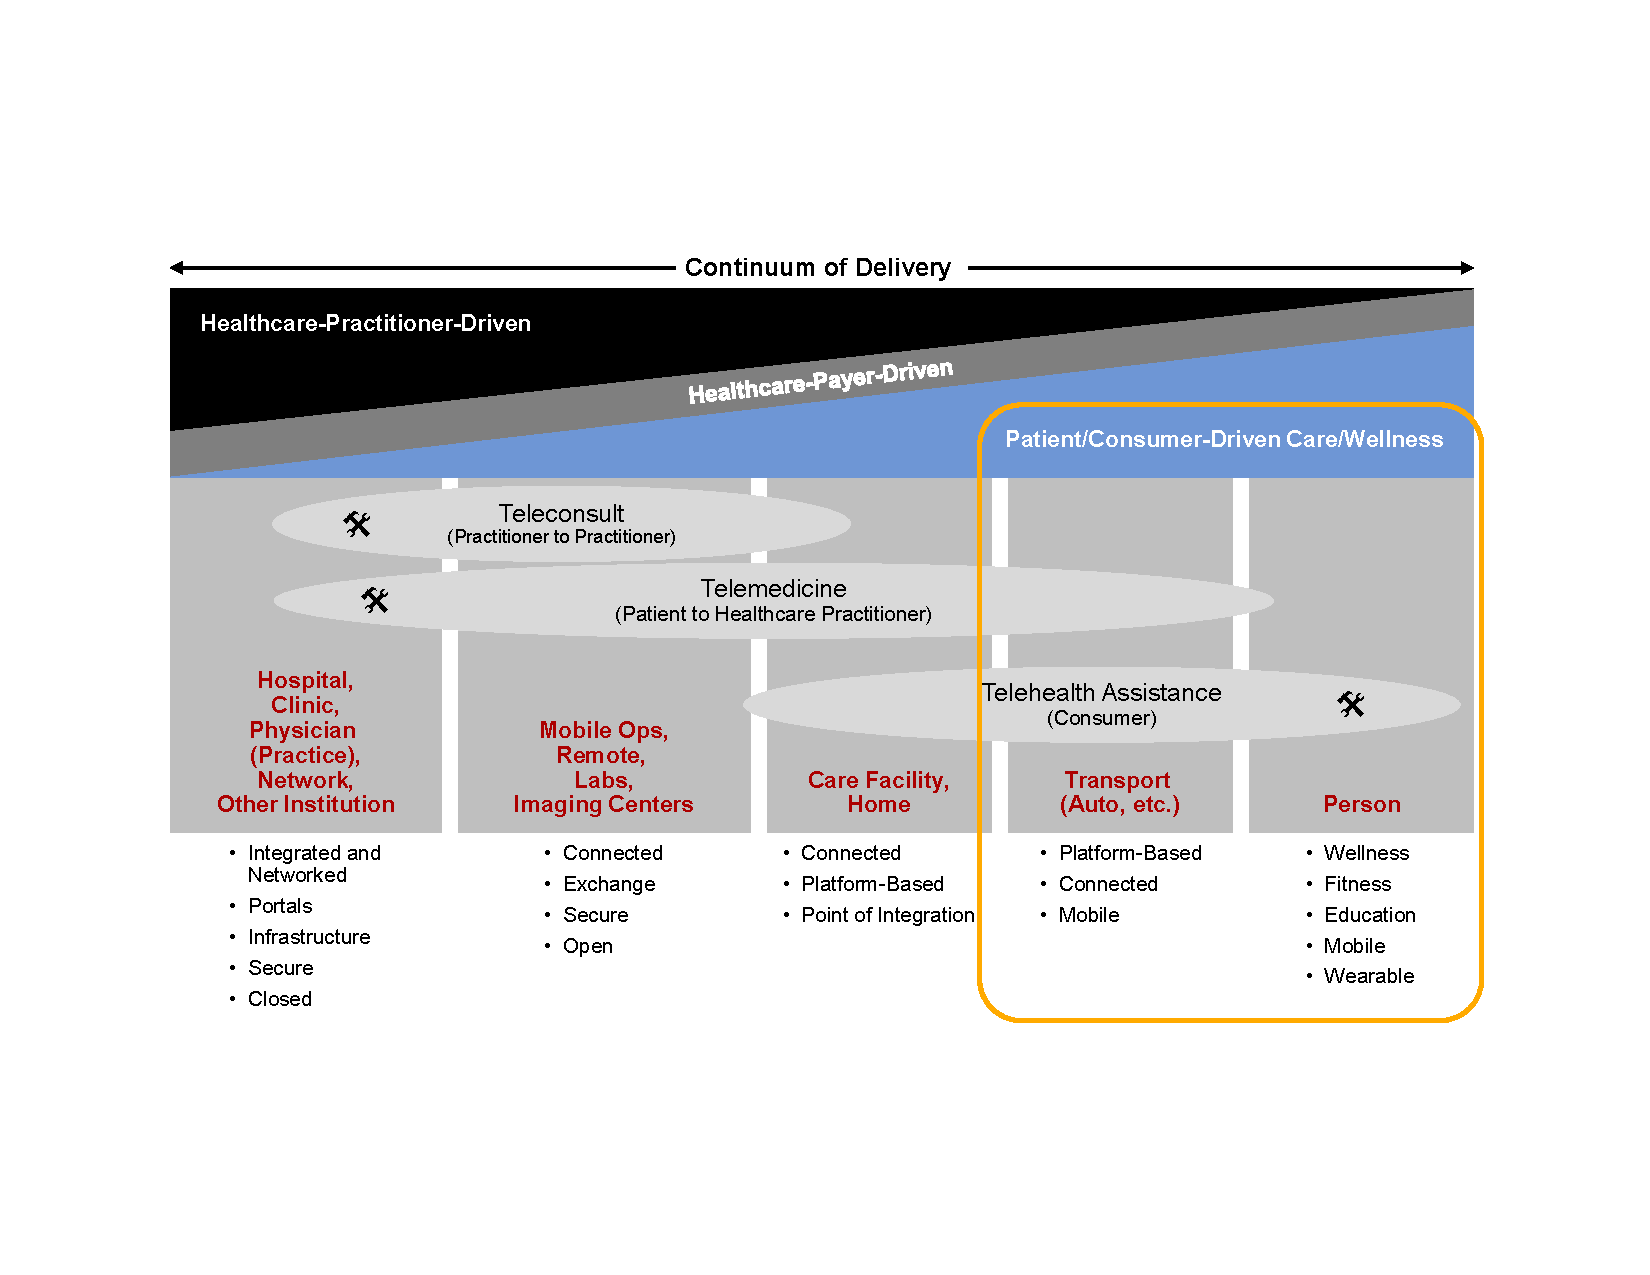
\includegraphics[width=.8\textwidth]{figures/continuum}
\caption{{Focus of Open mHealth network environment shown in yellow box. Figure from Gartner, 2013.  }}
% A Framework for Understanding Telehealth, Telemedicine and Other Remote Healthcare Delivery Solutions
% need to redraw before release
\label{fig:continuum}
\end{center}
\end{figure*}

\begin{figure}
\begin{center}
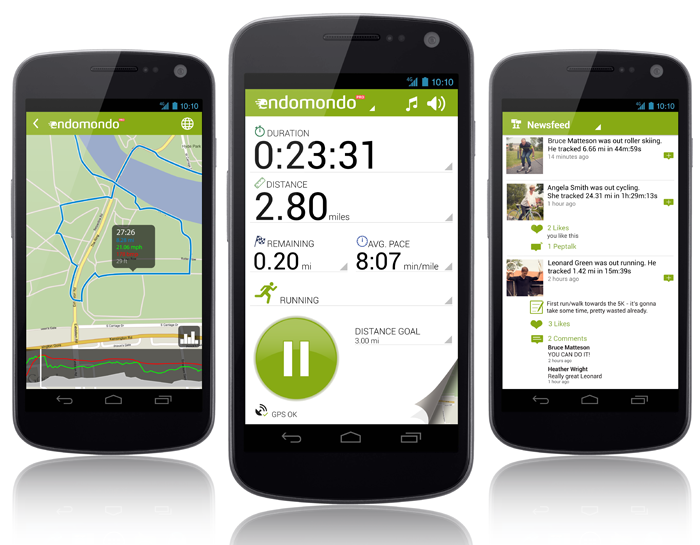
\includegraphics[width=.6\textwidth]{figures/endomondo}
\caption{Endomondo commercial fitness tracker. \protect\url{https://www.endomondo.com/}}
\label{fig:endomondo}
\end{center}
\end{figure}

\begin{figure}
\begin{center}
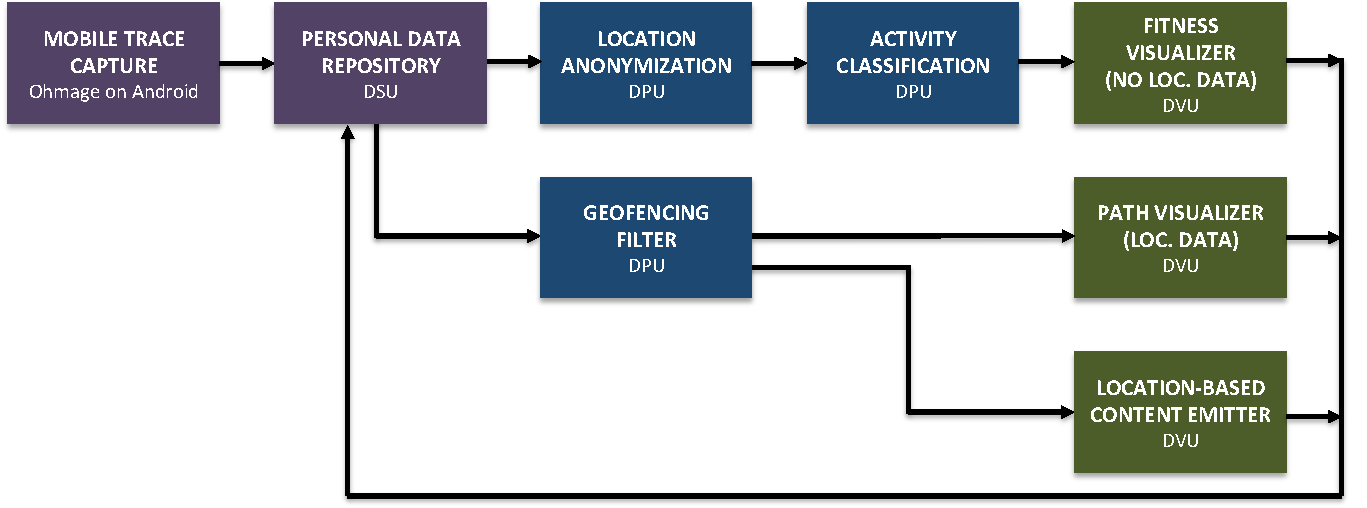
\includegraphics[width=1\textwidth]{figures/ConceptualBlock}
\caption{Conceptual block diagram showing data flow.}
\label{fig:ConceptualBlock}
\end{center}
\end{figure}

